\documentclass[a4paper, 14pt]{extarticle}

% Поля
%--------------------------------------
\usepackage{geometry}
\geometry{a4paper,tmargin=2cm,bmargin=2cm,lmargin=3cm,rmargin=1cm}
%--------------------------------------


%Russian-specific packages
%--------------------------------------
\usepackage[T2A]{fontenc}
\usepackage[utf8]{inputenc} 
\usepackage[english, main=russian]{babel}
%--------------------------------------

\usepackage{textcomp}

% Красная строка
%--------------------------------------
\usepackage{indentfirst}               
%--------------------------------------             


%Graphics
%--------------------------------------
\usepackage{graphicx}
\graphicspath{ {./images/} }
\usepackage{wrapfig}
%--------------------------------------

% Полуторный интервал
%--------------------------------------
\linespread{1.3}                    
%--------------------------------------

%Выравнивание и переносы
%--------------------------------------
% Избавляемся от переполнений
\sloppy
% Запрещаем разрыв страницы после первой строки абзаца
\clubpenalty=10000
% Запрещаем разрыв страницы после последней строки абзаца
\widowpenalty=10000
%--------------------------------------

%Списки
\usepackage{enumitem}

%Подписи
\usepackage{caption} 

%Гиперссылки
\usepackage{hyperref}

\hypersetup {
	unicode=true
}

%Рисунки
%--------------------------------------
\DeclareCaptionLabelSeparator*{emdash}{~--- }
\captionsetup[figure]{labelsep=emdash,font=onehalfspacing,position=bottom}
%--------------------------------------

\usepackage{tempora}

%Листинги
%--------------------------------------
\usepackage{listings}
\lstset{
  basicstyle=\ttfamily\footnotesize, 
  %basicstyle=\footnotesize\AnkaCoder,        % the size of the fonts that are used for the code
  breakatwhitespace=false,         % sets if automatic breaks shoulbd only happen at whitespace
  breaklines=true,                 % sets automatic line breaking
  captionpos=t,                    % sets the caption-position to bottom
  inputencoding=utf8,
  frame=single,                    % adds a frame around the code
  keepspaces=true,                 % keeps spaces in text, useful for keeping indentation of code (possibly needs columns=flexible)
  keywordstyle=\bf,       % keyword style
  numbers=left,                    % where to put the line-numbers; possible values are (none, left, right)
  numbersep=5pt,                   % how far the line-numbers are from the code
  xleftmargin=25pt,
  xrightmargin=25pt,
  showspaces=false,                % show spaces everywhere adding particular underscores; it overrides 'showstringspaces'
  showstringspaces=false,          % underline spaces within strings only
  showtabs=false,                  % show tabs within strings adding particular underscores
  stepnumber=1,                    % the step between two line-numbers. If it's 1, each line will be numbered
  tabsize=2,                       % sets default tabsize to 8 spaces
  title=\lstname                   % show the filename of files included with \lstinputlisting; also try caption instead of title
}
%--------------------------------------

%%% Математические пакеты %%%
%--------------------------------------
\usepackage{amsthm,amsfonts,amsmath,amssymb,amscd}  % Математические дополнения от AMS
\usepackage{mathtools}                              % Добавляет окружение multlined
\usepackage[perpage]{footmisc}
%--------------------------------------

%--------------------------------------
%			НАЧАЛО ДОКУМЕНТА
%--------------------------------------

\begin{document}

%--------------------------------------
%			ТИТУЛЬНЫЙ ЛИСТ
%--------------------------------------
\begin{titlepage}
\thispagestyle{empty}
\newpage


%Шапка титульного листа
%--------------------------------------
\vspace*{-60pt}
\hspace{-65pt}
\begin{minipage}{0.3\textwidth}
\hspace*{-20pt}\centering

\includegraphics[width=\textwidth]{emblem}
\end{minipage}
\begin{minipage}{0.67\textwidth}\small \textbf{
\vspace*{-0.7ex}
\hspace*{-6pt}\centerline{Министерство науки и высшего образования Российской Федерации}
\vspace*{-0.7ex}
\centerline{Федеральное государственное бюджетное образовательное учреждение }
\vspace*{-0.7ex}
\centerline{высшего образования}
\vspace*{-0.7ex}
\centerline{<<Московский государственный технический университет}
\vspace*{-0.7ex}
\centerline{имени Н.Э. Баумана}
\vspace*{-0.7ex}
\centerline{(национальный исследовательский университет)>>}
\vspace*{-0.7ex}
\centerline{(МГТУ им. Н.Э. Баумана)}}
\end{minipage}
%--------------------------------------

%Полосы
%--------------------------------------
\vspace{-25pt}
\hspace{-35pt}\rule{\textwidth}{2.3pt}

\vspace*{-20.3pt}
\hspace{-35pt}\rule{\textwidth}{0.4pt}
%--------------------------------------

\vspace{1.5ex}
\hspace{-35pt} \noindent \small ФАКУЛЬТЕТ\hspace{80pt} <<Информатика и системы управления>>

\vspace*{-16pt}
\hspace{47pt}\rule{0.83\textwidth}{0.4pt}

\vspace{0.5ex}
\hspace{-35pt} \noindent \small КАФЕДРА\hspace{50pt} <<Теоретическая информатика и компьютерные технологии>>

\vspace*{-16pt}
\hspace{30pt}\rule{0.866\textwidth}{0.4pt}
  
\vspace{11em}

\begin{center}
\Large {\bf Лабораторная работа № 5} \\
\large {\bf по курсу <<Теория искусственных нейронных сетей>>} \\
\large {\bf <<Сверточные нейронные сети (CNN)>>} \\
\end{center}\normalsize

\vspace{8em}


\begin{flushright}
  {Студентка группы ИУ9-72Б Самохвалова П. С. \hspace*{15pt}\\
  \vspace{2ex}
  Преподаватель Каганов Ю. Т.\hspace*{15pt}}
\end{flushright}

\bigskip

\vfill
 

\begin{center}
\textsl{Москва 2023}
\end{center}
\end{titlepage}
%--------------------------------------
%		КОНЕЦ ТИТУЛЬНОГО ЛИСТА
%--------------------------------------

\renewcommand{\ttdefault}{pcr}

\setlength{\tabcolsep}{3pt}
\newpage
\setcounter{page}{2}

\section{Задание}\label{Sect::task}

\begin{enumerate}
    \item Реализовать нейронную сеть LeNet. В качестве базы данных использовать MNIST. Применить оптимизаторы SGD, AdaDelta, NAG, Adam.
    \item Реализовать нейронную сеть VGG16. В качестве базы данных использовать CIFAR-10. Применить оптимизаторы SGD, AdaDelta, NAG, Adam.
    \item Реализовать нейронную сеть ResNet (34). В качестве базы данных использовать ImageNet. Применить оптимизаторы SGD, AdaDelta, NAG, Adam.
\end{enumerate}

\section{Практическая реализация}\label{Sect::code}

Исходный код программы представлен в листингах~\ref{lst:code1}-~\ref{lst:code3}.   

\begin{lstlisting}[language={python},caption={LeNet},label={lst:code1}]
import torch
import torch.nn as nn
import torch.optim as optim
import torchvision
import torchvision.transforms as transforms
from torch.utils.data import DataLoader
import torch.nn.functional as F
import matplotlib.pyplot as plt


transform = transforms.Compose([
    transforms.ToTensor(),
    transforms.Normalize((0.1307,), (0.3081,))
])


trainset = torchvision.datasets.MNIST(root='./data', train=True, download=True, transform=transform)
testset = torchvision.datasets.MNIST(root='./data', train=False, download=True, transform=transform)

trainloader = DataLoader(trainset, batch_size=64, shuffle=True)
testloader = DataLoader(testset, batch_size=64, shuffle=False)


class LeNet(nn.Module):
    def __init__(self):
        super(LeNet, self).__init__()
        self.conv1 = nn.Conv2d(1, 6, kernel_size=5)
        self.conv2 = nn.Conv2d(6, 16, kernel_size=5)
        self.fc1 = nn.Linear(16*4*4, 120)
        self.fc2 = nn.Linear(120, 84)
        self.fc3 = nn.Linear(84, 10)

    def forward(self, x):
        x = F.relu(self.conv1(x))
        x = F.max_pool2d(x, 2)
        x = F.relu(self.conv2(x))
        x = F.max_pool2d(x, 2)
        x = x.view(-1, 16*4*4)
        x = F.relu(self.fc1(x))
        x = F.relu(self.fc2(x))
        x = self.fc3(x)
        return x


model = LeNet()

criterion = nn.CrossEntropyLoss()

optimizer_sgd = optim.SGD(model.parameters(), lr=0.01, momentum=0.9)
optimizer_adadelta = optim.Adadelta(model.parameters())
optimizer_nag = optim.SGD(model.parameters(), lr=0.01, momentum=0.9, nesterov=True)
optimizer_adam = optim.Adam(model.parameters())


def train_test_model(optimizer, name):
    model.train()
    losses = []
    for epoch in range(10):
        running_loss = 0.0
        for i, data in enumerate(trainloader, 0):
            inputs, labels = data
            optimizer.zero_grad()
            outputs = model(inputs)
            loss = criterion(outputs, labels)
            loss.backward()
            optimizer.step()
            running_loss += loss.item()
        epoch_loss = running_loss / len(trainloader)
        losses.append(epoch_loss)
        print(f"{name} - Epoch {epoch + 1} loss: {epoch_loss}")

    model.eval()
    correct = 0
    total = 0
    with torch.no_grad():
        for data in testloader:
            images, labels = data
            outputs = model(images)
            _, predicted = torch.max(outputs, 1)
            total += labels.size(0)
            correct += (predicted == labels).sum().item()
    accuracy = 100 * correct / total
    print(f"{name} - Accuracy: {accuracy}%")

    return losses


sgd_losses = train_test_model(optimizer_sgd, "SGD")
adadelta_losses = train_test_model(optimizer_adadelta, "AdaDelta")
nag_losses = train_test_model(optimizer_nag, "NAG")
adam_losses = train_test_model(optimizer_adam, "Adam")


epochs = range(1, 11)
plt.plot(epochs, sgd_losses, label='SGD')
plt.plot(epochs, adadelta_losses, label='AdaDelta')
plt.plot(epochs, nag_losses, label='NAG')
plt.plot(epochs, adam_losses, label='Adam')
plt.xlabel('Epoch')
plt.ylabel('Loss')
plt.title('Loss function dependence on the number of epochs for each optimizer')
plt.legend()
plt.show()

\end{lstlisting}

\begin{lstlisting}[language={python},caption={VGG16},label={lst:code2}]
import torch
import torch.nn as nn
import torch.optim as optim
import torchvision
import torchvision.transforms as transforms
import matplotlib.pyplot as plt

model = torchvision.models.vgg16(pretrained=False)

num_classes = 10
model.classifier[6] = nn.Linear(4096, num_classes)

device = torch.device("cuda:0" if torch.cuda.is_available() else "cpu")
model.to(device)

transform = transforms.Compose(
    [
        transforms.ToTensor(),
        transforms.Normalize((0.5, 0.5, 0.5), (0.5, 0.5, 0.5))
    ]
)

trainset = torchvision.datasets.CIFAR10(root='./data', train=True, download=True, transform=transform)
trainloader = torch.utils.data.DataLoader(trainset, batch_size=4, shuffle=True, num_workers=2)

testset = torchvision.datasets.CIFAR10(root='./data', train=False, download=True, transform=transform)
testloader = torch.utils.data.DataLoader(testset, batch_size=4, shuffle=False, num_workers=2)

optimizers = {
    "SGD": optim.SGD(model.parameters(), lr=0.001, momentum=0.9),
    "AdaDelta": optim.Adadelta(model.parameters(), lr=0.01),
    "NAG": optim.SGD(model.parameters(), lr=0.001, momentum=0.9, nesterov=True),
    "Adam": optim.Adam(model.parameters(), lr=0.00001)
}

for optimizer_name, optimizer in optimizers.items():
    criterion = nn.CrossEntropyLoss()
    epochs = 5

    optimizer_losses = [0] * epochs

    for epoch in range(epochs):
        running_loss = 0
        for i, data in enumerate(trainloader, 0):
            inputs, labels = data
            inputs, labels = inputs.to(device), labels.to(device)

            optimizer.zero_grad()

            outputs = model(inputs)
            loss = criterion(outputs, labels)
            loss.backward()
            optimizer.step()

            running_loss += loss.item()

            optimizer_losses[epoch] += loss.item()

            if i % 2000 == 1999:
                print(f"[{optimizer_name}, {epoch + 1}, {i + 1}] loss: {running_loss / 2000}")
                running_loss = 0.0

        optimizer_losses[epoch] /= len(trainloader)

    correct = 0
    total = 0
    with torch.no_grad():
        for data in testloader:
            images, labels = data
            images, labels = images.to(device), labels.to(device)
            outputs = model(images)
            _, predicted = torch.max(outputs, 1)
            total += labels.size(0)
            correct += (predicted == labels).sum().item()

    print(f"Accuracy of the network with {optimizer_name} optimizer: {100 * correct / total}%")

    plt.plot(range(1, epochs + 1), optimizer_losses, label=optimizer_name)
    plt.xlabel('Epoch')
    plt.ylabel('Loss')
    plt.title('Loss function dependence on the number of epochs for optimizer ' + optimizer_name)
    plt.legend()
    plt.show()


\end{lstlisting}

\begin{lstlisting}[language={python},caption={ResNet (34)},label={lst:code3}]
import torch
import torch.nn as nn
import torch.optim as optim
import torchvision.transforms as transforms
import torchvision.datasets as datasets
import torchvision.models as models
import matplotlib.pyplot as plt


device = torch.device("cuda" if torch.cuda.is_available() else "cpu")


transform = transforms.Compose([
    transforms.Resize(256),
    transforms.CenterCrop(224),
    transforms.ToTensor(),
    transforms.Normalize(mean=[0.485, 0.456, 0.406], std=[0.229, 0.224, 0.225])
])


train_dataset = datasets.CIFAR10(root='./data', train=True, download=True, transform=transform)
test_dataset = datasets.CIFAR10(root='./data', train=False, download=True, transform=transform)


train_loader = torch.utils.data.DataLoader(dataset=train_dataset, batch_size=64, shuffle=True)
test_loader = torch.utils.data.DataLoader(dataset=test_dataset, batch_size=64, shuffle=False)


model = models.resnet34(pretrained=False)
model.to(device)


criterion = nn.CrossEntropyLoss()


accuracies = {}


optimizers = ['SGD', 'Adadelta', 'NAG', 'Adam']
losses = {optimizer_name: [] for optimizer_name in optimizers}

for optimizer_name in optimizers:
    if optimizer_name == 'SGD':
        optimizer = optim.SGD(model.parameters(), lr=0.01, momentum=0.9)
    elif optimizer_name == 'Adadelta':
        optimizer = optim.Adadelta(model.parameters())
    elif optimizer_name == 'NAG':
        optimizer = optim.SGD(model.parameters(), lr=0.01, momentum=0.9, nesterov=True)
    elif optimizer_name == 'Adam':
        optimizer = optim.Adam(model.parameters(), lr=0.001)

    for epoch in range(5):
        model.train()
        running_loss = 0.0
        for images, labels in train_loader:
            images, labels = images.to(device), labels.to(device)
            optimizer.zero_grad()
            outputs = model(images)
            loss = criterion(outputs, labels)
            loss.backward()
            optimizer.step()
            running_loss += loss.item()
        print(f"Epoch {epoch+1}, Optimizer: {optimizer_name}, Loss: {running_loss / len(train_loader)}")
        losses[optimizer_name].append(running_loss / len(train_loader))

    model.eval()
    correct = 0
    total = 0
    with torch.no_grad():
        for images, labels in test_loader:
            images, labels = images.to(device), labels.to(device)
            outputs = model(images)
            _, predicted = torch.max(outputs, 1)
            total += labels.size(0)
            correct += (predicted == labels).sum().item()
    accuracy = 100 * correct / total
    accuracies[optimizer_name] = accuracy
    print(f'Accuracy of the network on the test images with {optimizer_name} optimizer: {accuracy:.2f}%')

    plt.plot(range(1, 6), losses[optimizer_name], label=optimizer_name)
    plt.xlabel('Epoch')
    plt.ylabel('Loss')
    plt.title('Loss function dependence on the number of epochs for optimizer ' + optimizer_name)
    plt.legend()
    plt.show()


print("Accuracies for different optimizers:")
for optimizer_name, accuracy in accuracies.items():
    print(f"{optimizer_name}: {accuracy:.2f}%")

\end{lstlisting}

\section{Результаты}\label{Sect::res}

Результаты работы программы представлены на рисунках~\ref{fig:img1}-~\ref{fig:img19}.

\begin{figure}[!htb]
	\centering
	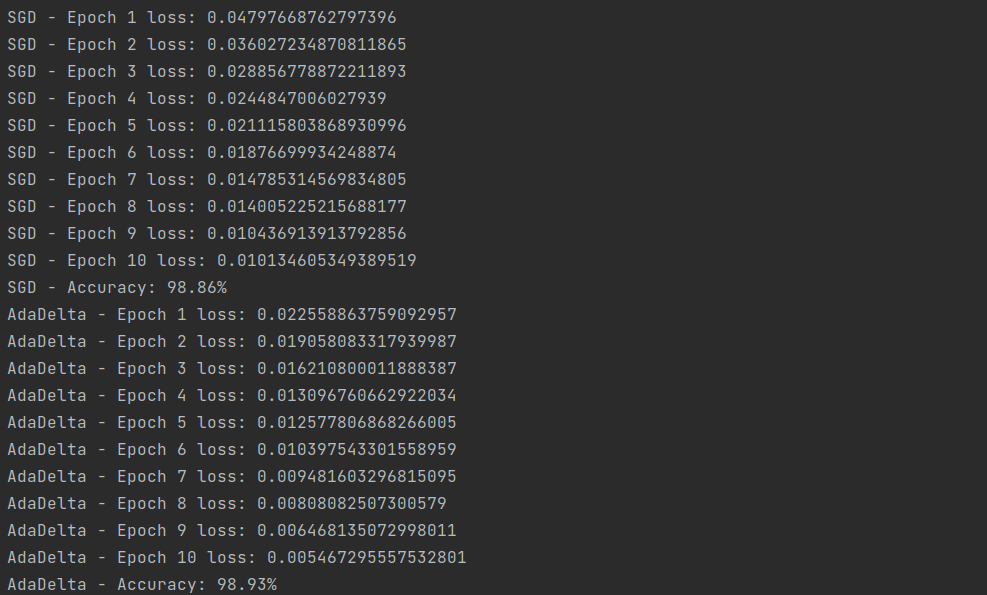
\includegraphics[width=0.8\textwidth]{img1}
\caption{Результат работы нейронной сети LeNet с оптимизаторами SGD и AdaDelta}
\label{fig:img1}
\end{figure}

\begin{figure}[!htb]
	\centering
	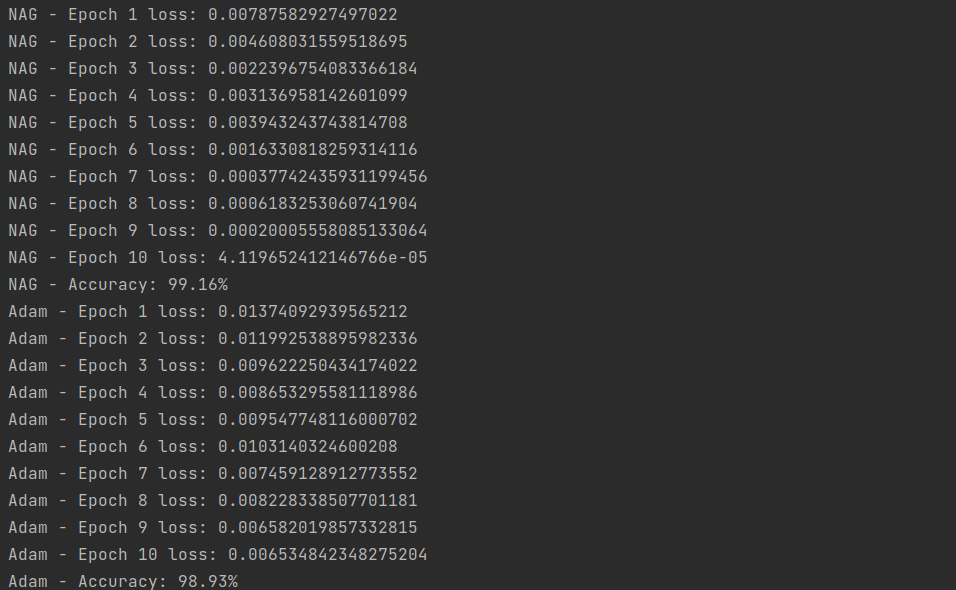
\includegraphics[width=0.8\textwidth]{img2}
\caption{Результат работы нейронной сети LeNet с оптимизаторами NAG и Adam}
\label{fig:img2}
\end{figure}

\begin{figure}[!htb]
	\centering
	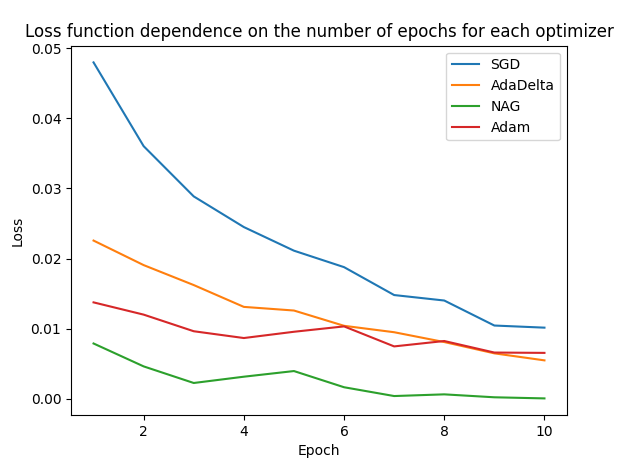
\includegraphics[width=0.8\textwidth]{img3}
\caption{Результат работы нейронной сети LeNet с оптимизаторами SGD, AdaDelta, NAG и Adam}
\label{fig:img3}
\end{figure}

\begin{figure}[!htb]
	\centering
	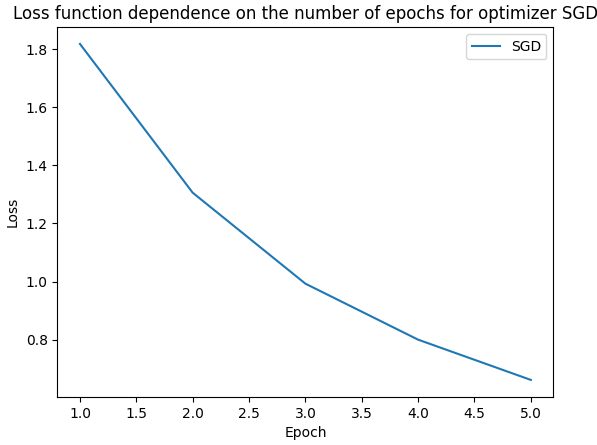
\includegraphics[width=0.8\textwidth]{img4}
\caption{Результат работы нейронной сети VGG16 с оптимизатором SGD}
\label{fig:img4}
\end{figure}

\begin{figure}[!htb]
	\centering
	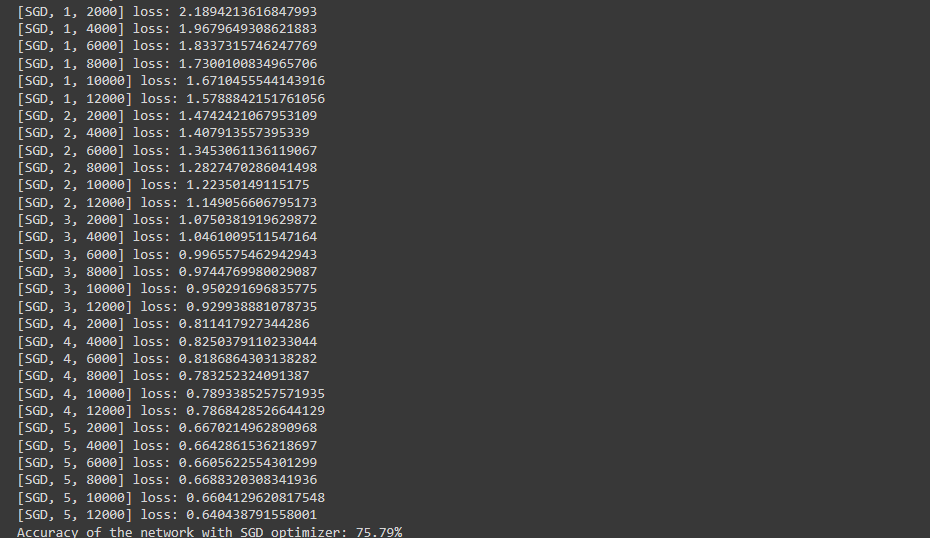
\includegraphics[width=0.8\textwidth]{img5}
\caption{Результат работы нейронной сети VGG16 с оптимизатором SGD}
\label{fig:img5}
\end{figure}

\begin{figure}[!htb]
	\centering
	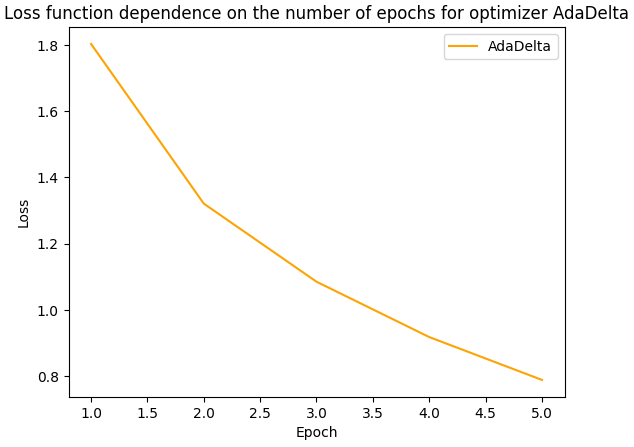
\includegraphics[width=0.8\textwidth]{img6}
\caption{Результат работы нейронной сети VGG16 с оптимизатором AdaDelta}
\label{fig:img6}
\end{figure}

\begin{figure}[!htb]
	\centering
	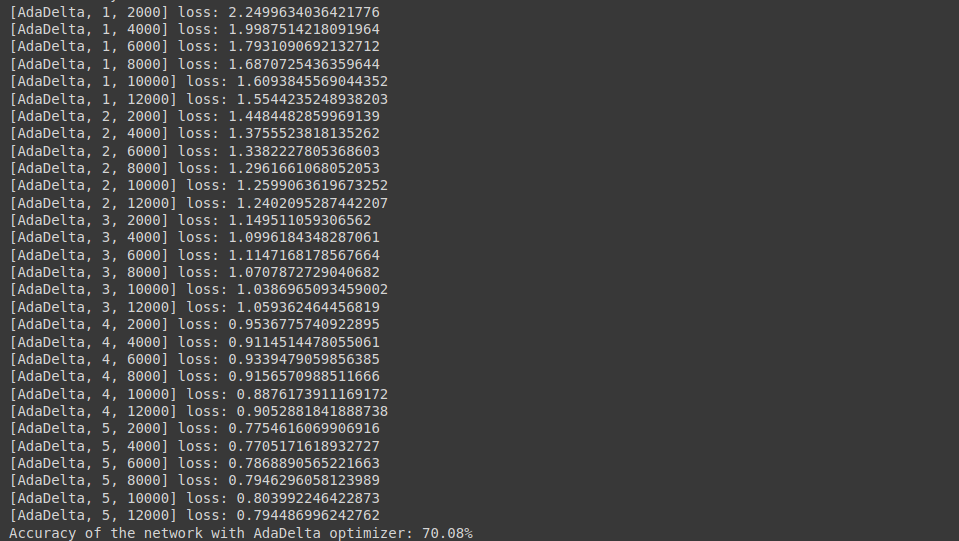
\includegraphics[width=0.8\textwidth]{img7}
\caption{Результат работы нейронной сети VGG16 с оптимизатором AdaDelta}
\label{fig:img7}
\end{figure}

\begin{figure}[!htb]
	\centering
	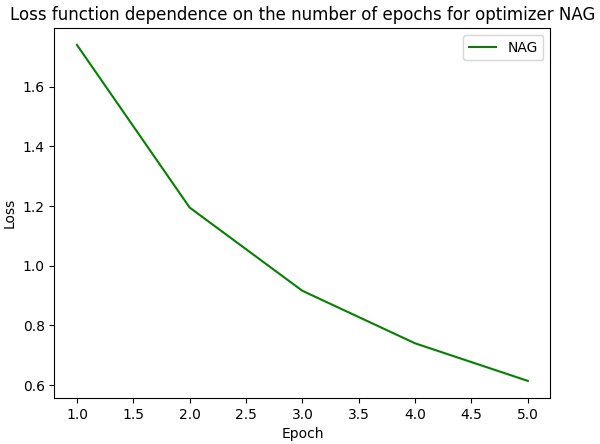
\includegraphics[width=0.8\textwidth]{img8}
\caption{Результат работы нейронной сети VGG16 с оптимизатором NAG}
\label{fig:img8}
\end{figure}

\begin{figure}[!htb]
	\centering
	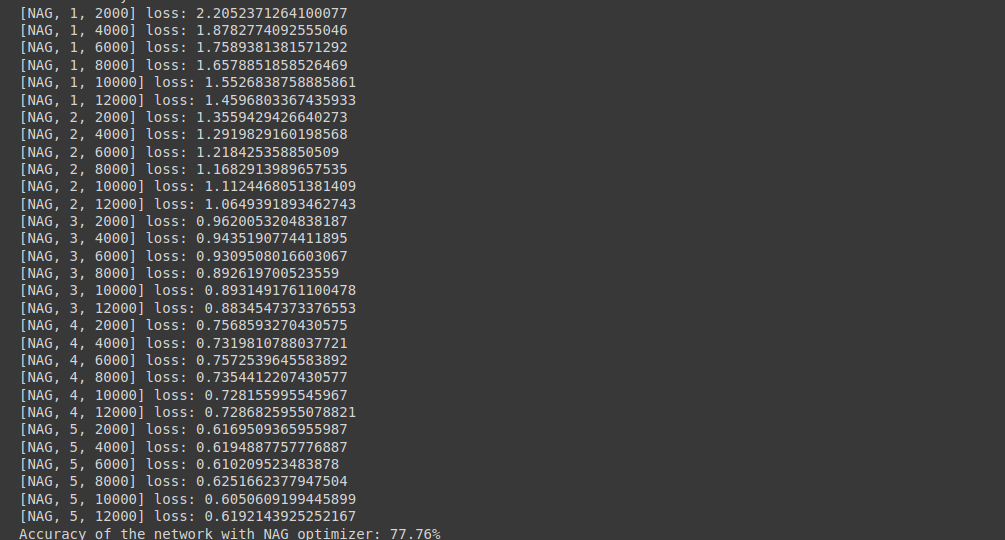
\includegraphics[width=0.8\textwidth]{img9}
\caption{Результат работы нейронной сети VGG16 с оптимизатором NAG}
\label{fig:img9}
\end{figure}

\begin{figure}[!htb]
	\centering
	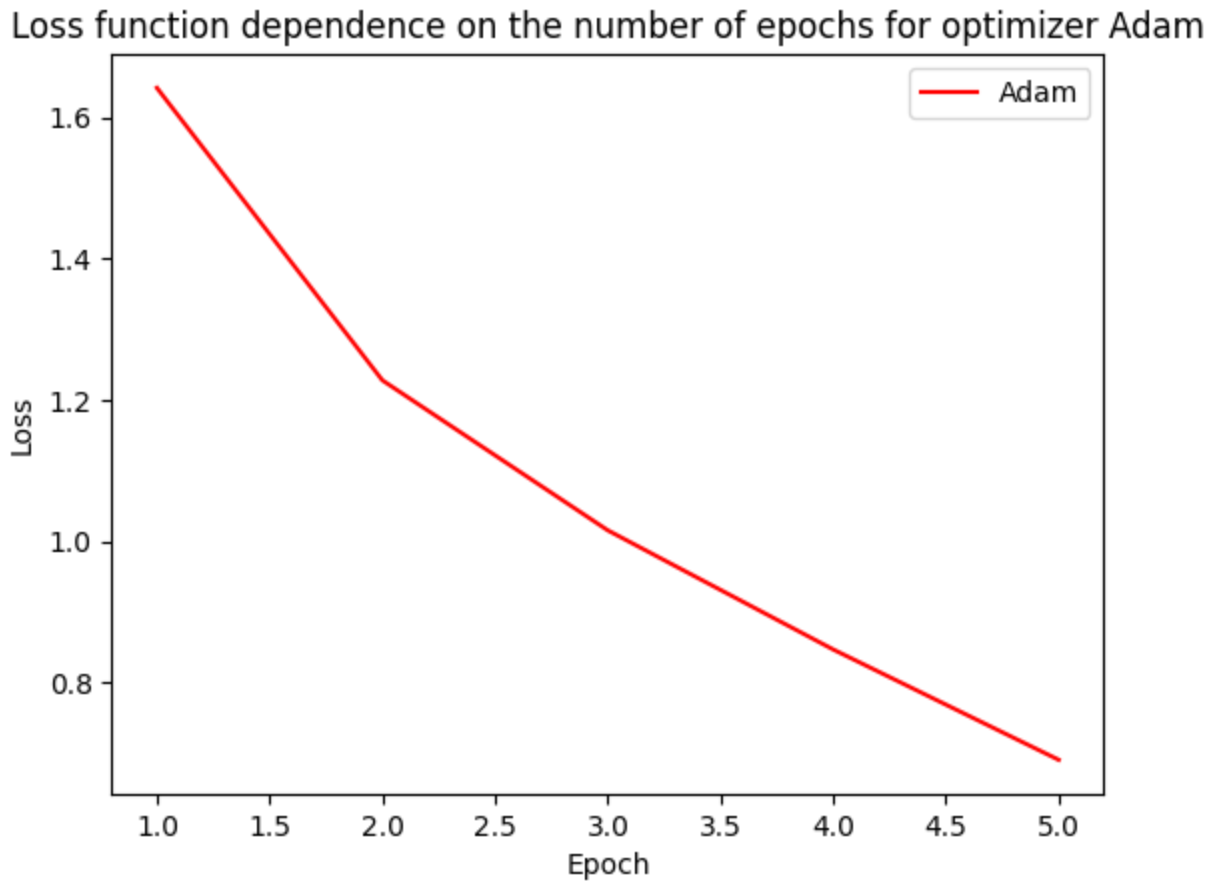
\includegraphics[width=0.8\textwidth]{img10}
\caption{Результат работы нейронной сети VGG16 с оптимизатором Adam}
\label{fig:img10}
\end{figure}

\begin{figure}[!htb]
	\centering
	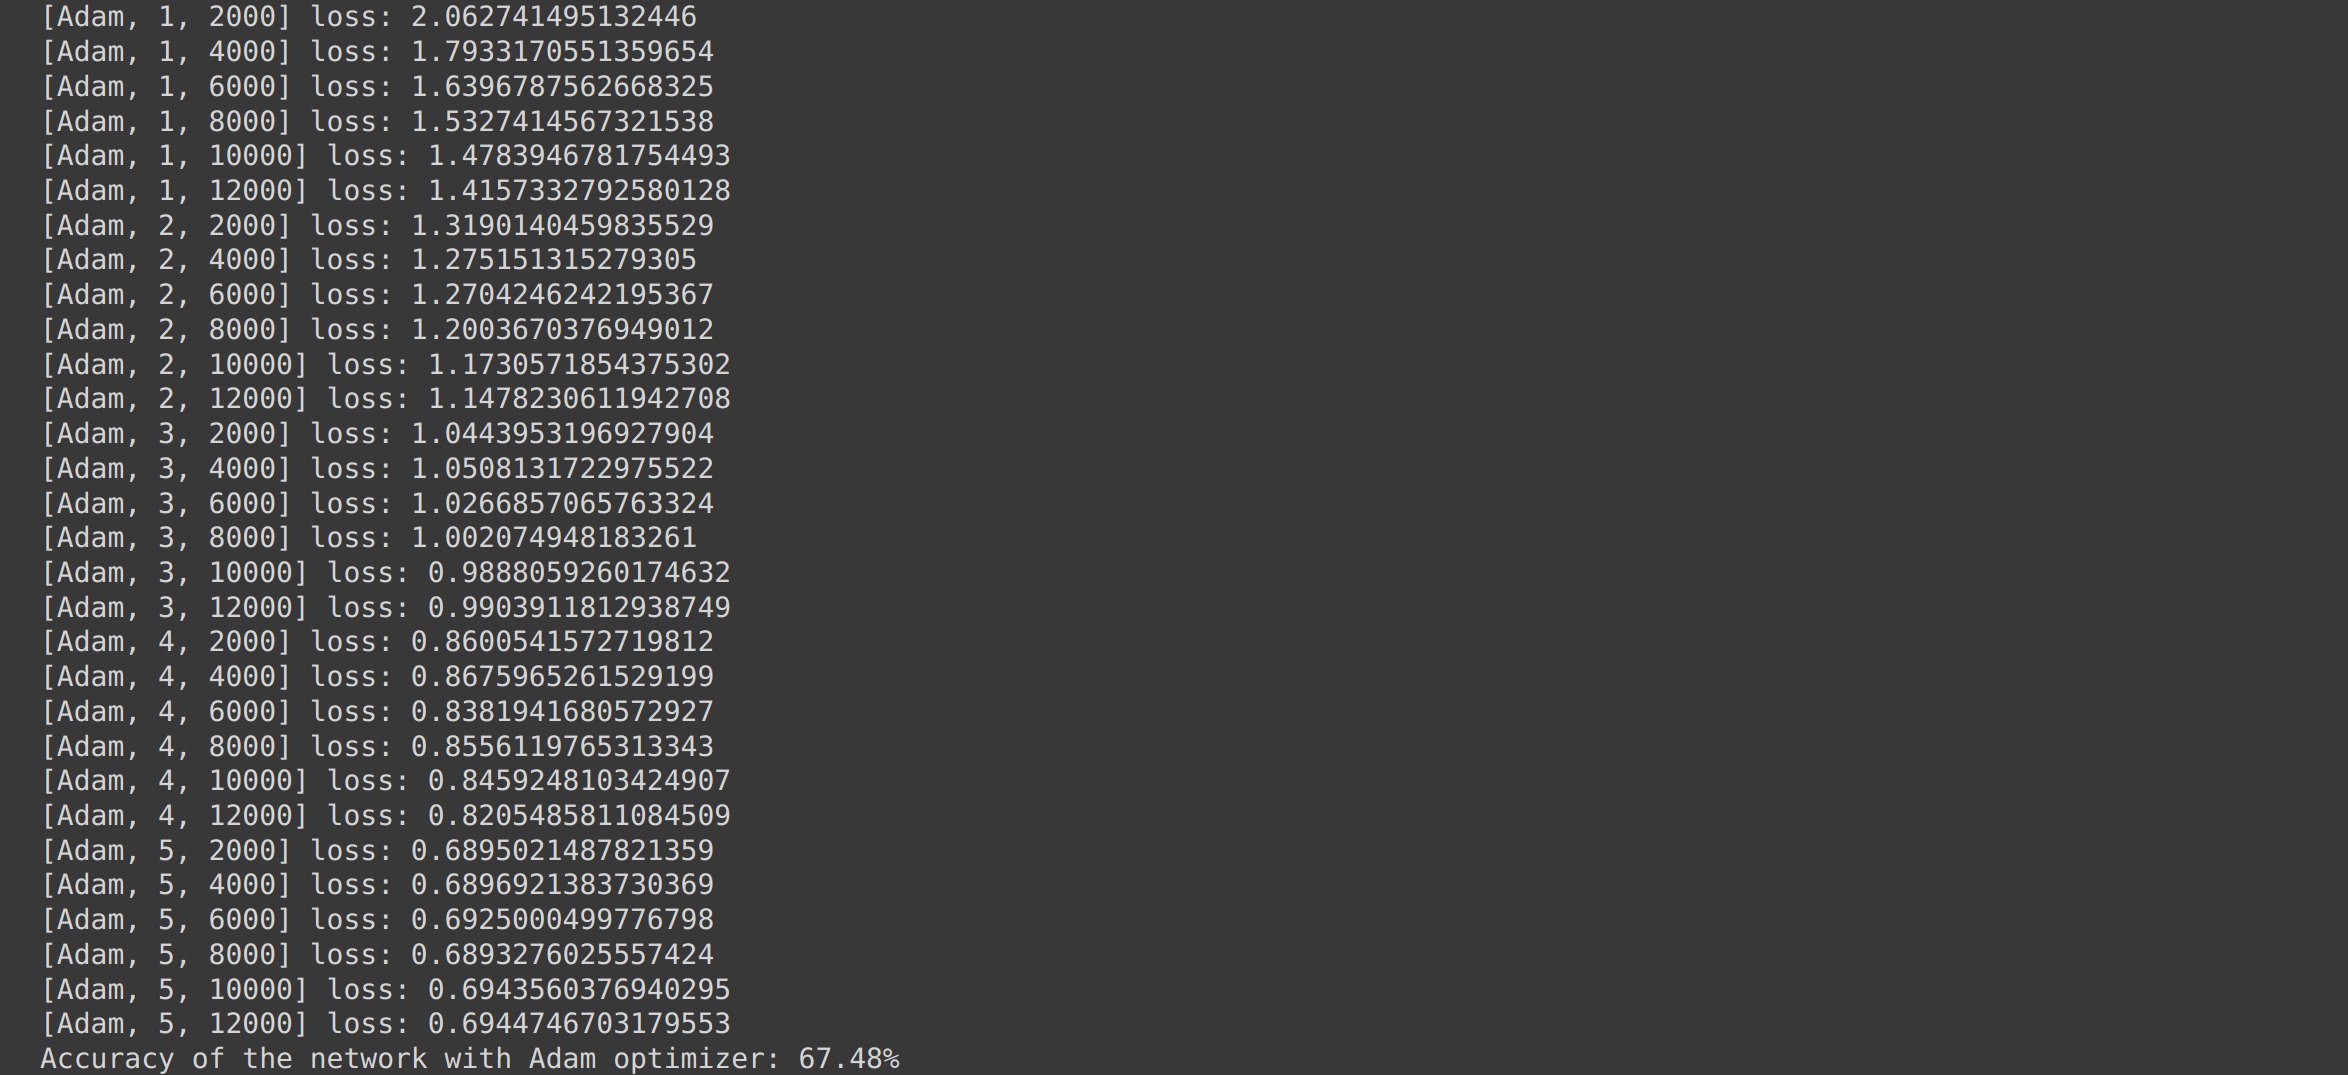
\includegraphics[width=0.8\textwidth]{img11}
\caption{Результат работы нейронной сети VGG16 с оптимизатором Adam}
\label{fig:img11}
\end{figure}

\begin{figure}[!htb]
	\centering
	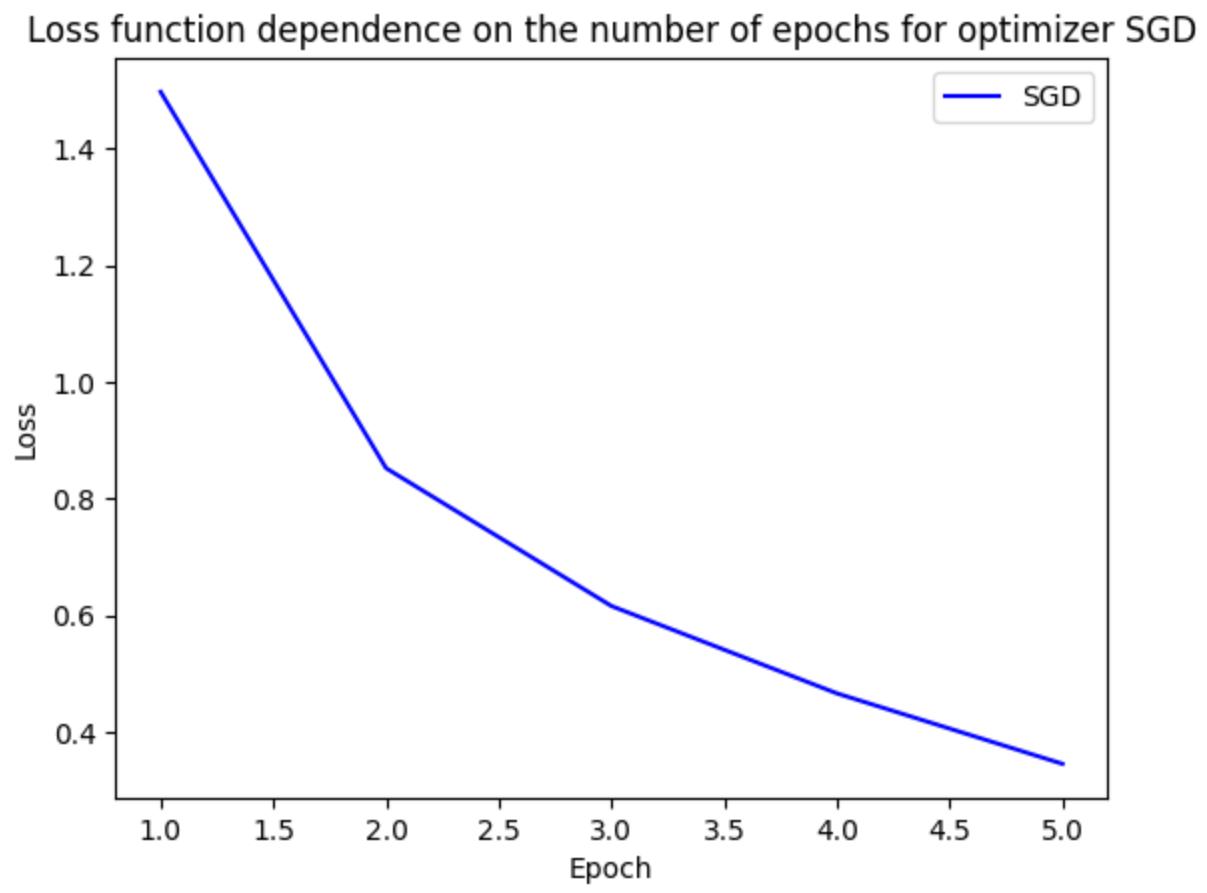
\includegraphics[width=0.8\textwidth]{img12}
\caption{Результат работы нейронной сети ResNet (34) с оптимизатором SGD}
\label{fig:img12}
\end{figure}

\begin{figure}[!htb]
	\centering
	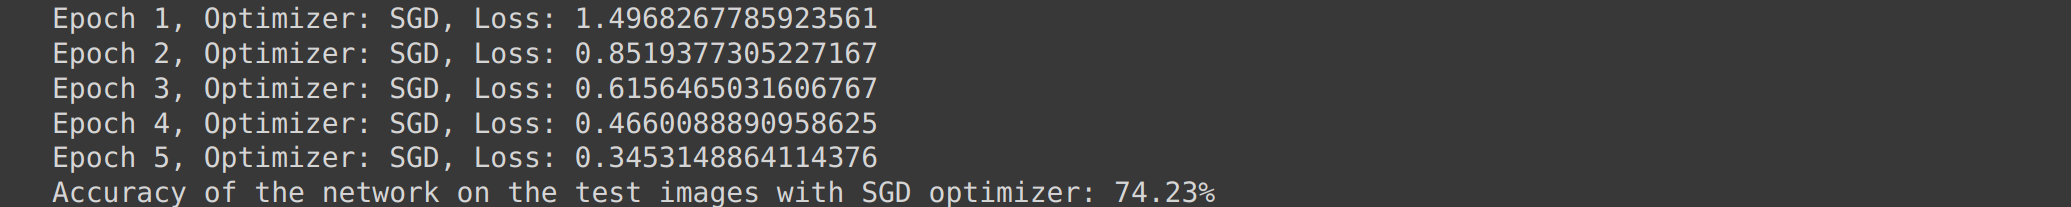
\includegraphics[width=0.8\textwidth]{img13}
\caption{Результат работы нейронной сети ResNet (34) с оптимизатором SGD}
\label{fig:img13}
\end{figure}

\begin{figure}[!htb]
	\centering
	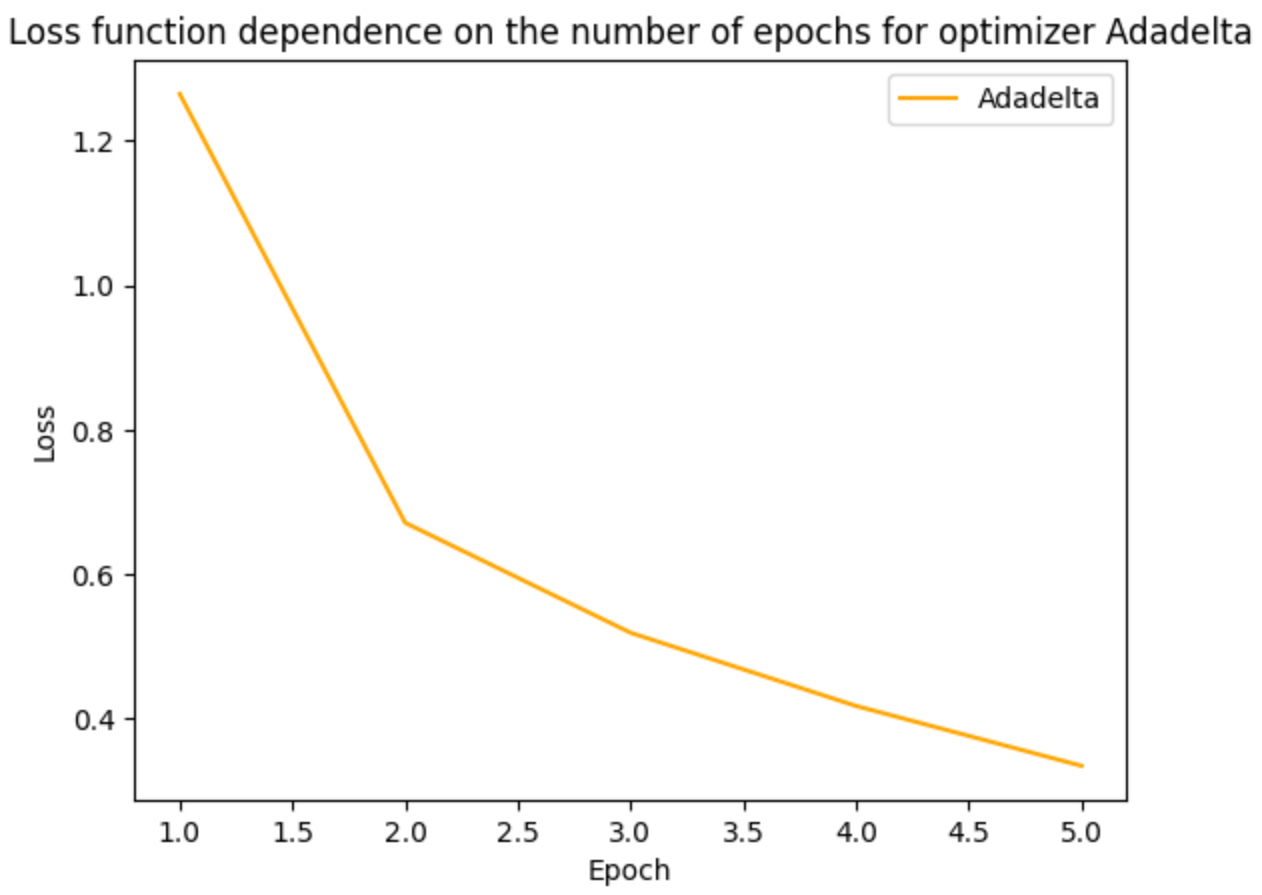
\includegraphics[width=0.8\textwidth]{img14}
\caption{Результат работы нейронной сети ResNet (34) с оптимизатором AdaDelta}
\label{fig:img14}
\end{figure}

\begin{figure}[!htb]
	\centering
	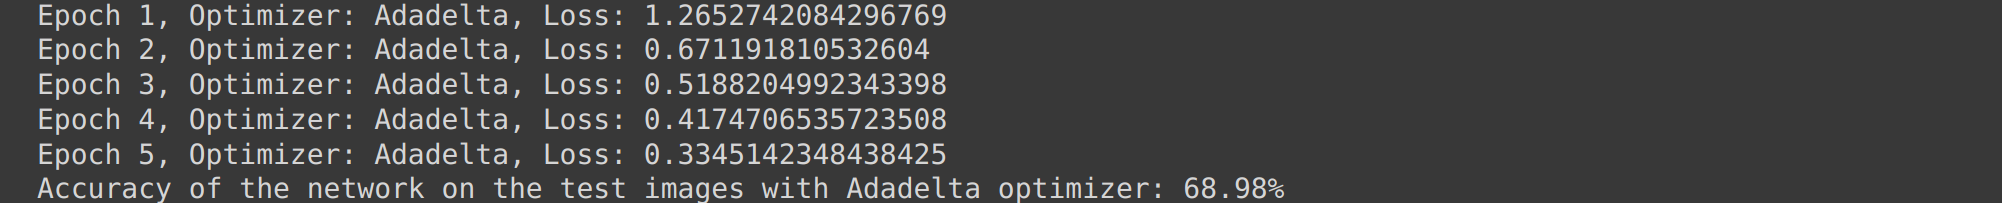
\includegraphics[width=0.8\textwidth]{img15}
\caption{Результат работы нейронной сети ResNet (34) с оптимизатором AdaDelta}
\label{fig:img15}
\end{figure}

\begin{figure}[!htb]
	\centering
	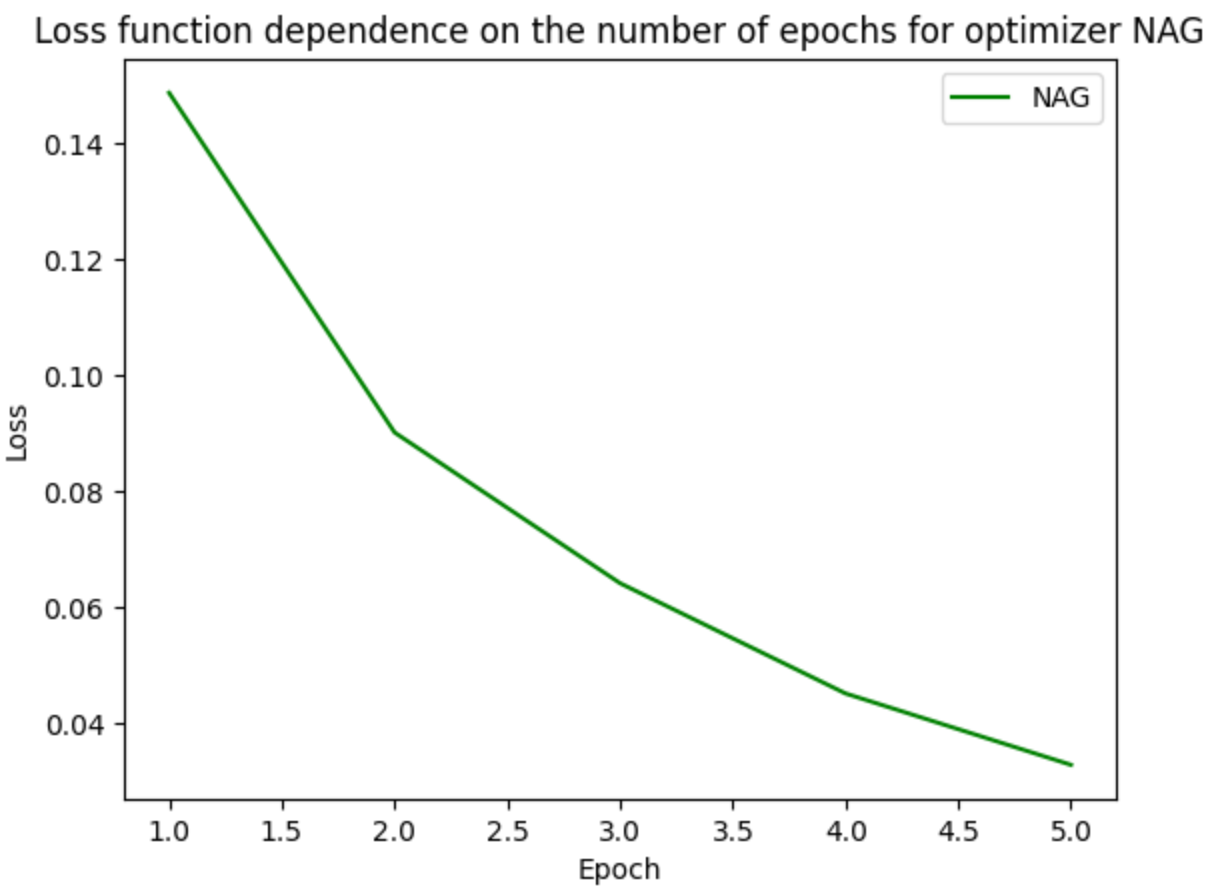
\includegraphics[width=0.8\textwidth]{img16}
\caption{Результат работы нейронной сети ResNet (34) с оптимизатором NAG}
\label{fig:img16}
\end{figure}

\begin{figure}[!htb]
	\centering
	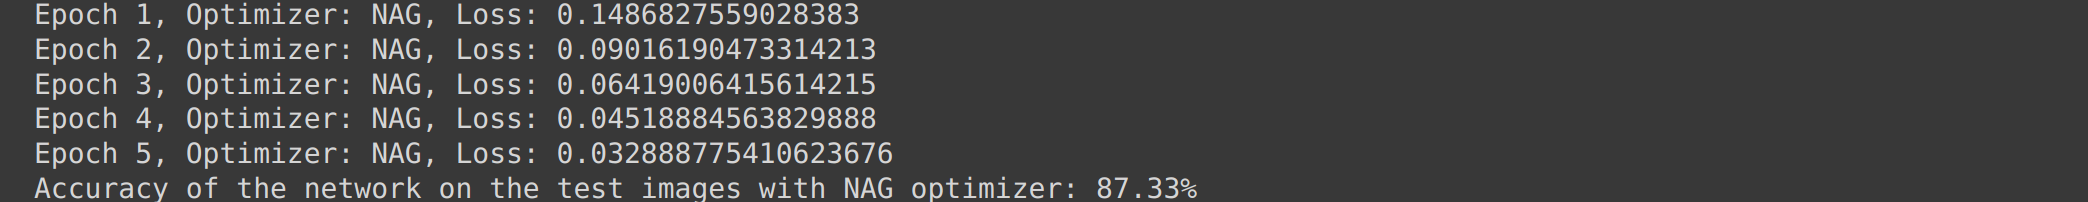
\includegraphics[width=0.8\textwidth]{img17}
\caption{Результат работы нейронной сети ResNet (34) с оптимизатором NAG}
\label{fig:img17}
\end{figure}

\begin{figure}[!htb]
	\centering
	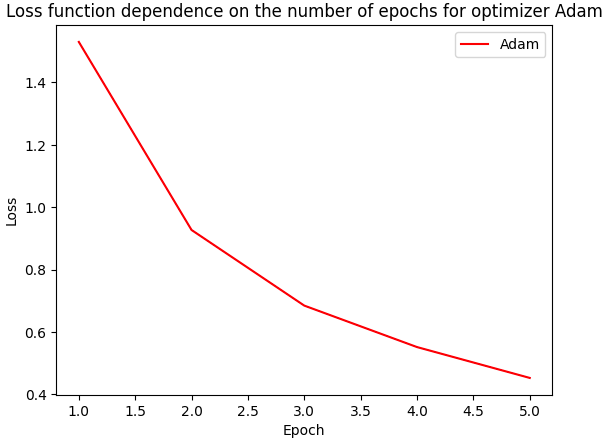
\includegraphics[width=0.8\textwidth]{img18}
\caption{Результат работы нейронной сети ResNet (34) с оптимизатором Adam}
\label{fig:img18}
\end{figure}

\begin{figure}[!htb]
	\centering
	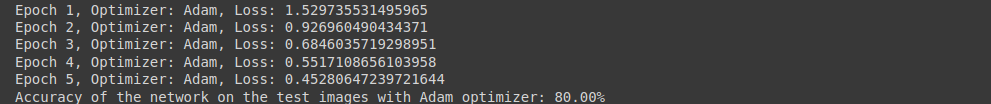
\includegraphics[width=0.8\textwidth]{img19}
\caption{Результат работы нейронной сети ResNet (34) с оптимизатором Adam}
\label{fig:img19}
\end{figure}

\section{Выводы}\label{Sect::conclusion}

В результате выполнения лабораторной работы на PyTorch были реализованы нейронные сети LeNet, VGG16, ResNet (34) с оптимизаторами SGD, AdaDelta, NAG, Adam.

\end{document}
